\documentclass[]{jarticle}          % 一段組
%\documentclass[twocolumn]{jarticle} % 二段組

\textwidth 180mm
\textheight 255mm
\oddsidemargin -12mm
\topmargin -15mm
\columnsep 10mm

%\vspace{0.5cm} % 一段組の場合はコメントアウトした方が体裁がよいx
%] % 一段組の場合はコメントアウトする

\usepackage{styles/labheadings}
\usepackage[dvipdfmx]{graphicx,color}
\usepackage{amsmath,amssymb}
\usepackage{url}
% 追加
\usepackage{listings,jvlisting}
\usepackage[hang,small,bf]{caption}
\usepackage[subrefformat=parens]{subcaption}
\captionsetup{compatibility=false}

\newcommand{\aU}{\mbox{\boldmath $a$}}
\newcommand{\bU}{\mbox{\boldmath $b$}}
\newcommand{\cU}{\mbox{\boldmath $c$}}
\newcommand{\dU}{\mbox{\boldmath $d$}}
\newcommand{\eU}{\mbox{\boldmath $e$}}
\newcommand{\fU}{\mbox{\boldmath $f$}}
\newcommand{\gU}{\mbox{\boldmath $g$}}
\newcommand{\hU}{\mbox{\boldmath $h$}}
\newcommand{\iU}{\mbox{\boldmath $i$}}
\newcommand{\jU}{\mbox{\boldmath $j$}}
\newcommand{\kU}{\mbox{\boldmath $k$}}
\newcommand{\lU}{\mbox{\boldmath $l$}}
\newcommand{\mU}{\mbox{\boldmath $m$}}
\newcommand{\nU}{\mbox{\boldmath $n$}}
\newcommand{\oU}{\mbox{\boldmath $o$}}
\newcommand{\pU}{\mbox{\boldmath $p$}}
\newcommand{\qU}{\mbox{\boldmath $q$}}
\newcommand{\rU}{\mbox{\boldmath $r$}}
\newcommand{\sU}{\mbox{\boldmath $s$}}
\newcommand{\tU}{\mbox{\boldmath $t$}}
\newcommand{\uU}{\mbox{\boldmath $u$}}
\newcommand{\vU}{\mbox{\boldmath $v$}}
\newcommand{\wU}{\mbox{\boldmath $w$}}
\newcommand{\xU}{\mbox{\boldmath $x$}}
\newcommand{\yU}{\mbox{\boldmath $y$}}
\newcommand{\zU}{\mbox{\boldmath $z$}}
\newcommand{\AU}{\mbox{\boldmath $A$}}
\newcommand{\BU}{\mbox{\boldmath $B$}}
\newcommand{\CU}{\mbox{\boldmath $C$}}
\newcommand{\DU}{\mbox{\boldmath $D$}}
\newcommand{\EU}{\mbox{\boldmath $E$}}
\newcommand{\FU}{\mbox{\boldmath $F$}}
\newcommand{\GU}{\mbox{\boldmath $G$}}
\newcommand{\HU}{\mbox{\boldmath $H$}}
\newcommand{\IU}{\mbox{\boldmath $I$}}
\newcommand{\JU}{\mbox{\boldmath $J$}}
\newcommand{\KU}{\mbox{\boldmath $K$}}
\newcommand{\LU}{\mbox{\boldmath $L$}}
\newcommand{\MU}{\mbox{\boldmath $M$}}
\newcommand{\NU}{\mbox{\boldmath $N$}}
\newcommand{\OU}{\mbox{\boldmath $O$}}
\newcommand{\PU}{\mbox{\boldmath $P$}}
\newcommand{\QU}{\mbox{\boldmath $Q$}}
\newcommand{\RU}{\mbox{\boldmath $R$}}
\newcommand{\SU}{\mbox{\boldmath $S$}}
\newcommand{\TU}{\mbox{\boldmath $T$}}
\newcommand{\UU}{\mbox{\boldmath $U$}}
\newcommand{\VU}{\mbox{\boldmath $V$}}
\newcommand{\WU}{\mbox{\boldmath $W$}}
\newcommand{\XU}{\mbox{\boldmath $X$}}
\newcommand{\YU}{\mbox{\boldmath $Y$}}
\newcommand{\ZU}{\mbox{\boldmath $Z$}}
\newcommand{\epU}{\mbox{\boldmath $\epsilon$}}
\newcommand{\taU}{\mbox{\boldmath $\tau$}}
\newcommand{\etU}{\mbox{\boldmath $\eta$}}
\newcommand{\xiU}{\mbox{\boldmath $\xi$}}
\newcommand{\wwU}{\mbox{\boldmath $\omega$}}
\newcommand{\WwU}{\mbox{\boldmath $\Omega$}}
\newcommand{\lmU}{\mbox{\boldmath $\lambda$}}
\newcommand{\LmU}{\mbox{\boldmath $\Lambda$}}
\newcommand{\PiU}{\mbox{\boldmath $\Pi$}}
\newcommand{\SgU}{\mbox{\boldmath $\Sigma$}}
\newcommand{\thU}{\mbox{\boldmath $\theta$}}
\newcommand{\ThU}{\mbox{\boldmath $\Theta$}}
\newcommand{\roU}{\mbox{\boldmath $\rho$}}
\newcommand{\nuU}{\mbox{\boldmath $\nu$}}
\newcommand{\ones}{{\bf 1}}
\newcommand{\zr}{{\bf 0}}
\newcommand{\eq}{\begin{equation}}
\newcommand{\en}{\end{equation}}
\newcommand{\eqa}{\begin{eqnarray}}
\newcommand{\ena}{\end{eqnarray}}
\newcommand{\xx}{\makebox[1cm]{}}
\newcommand{\xm}{\makebox[0.5cm]{}}
\newcommand{\x}{\makebox[0.2cm]{}}
\newcommand{\tr}{{\rm tr}}
\newcommand{\sgn}{{\rm sgn}}
\newcommand{\ad}{{\rm ad}}

\newcommand{\rank}{{\rm rank}}
\newcommand{\diag}{{\rm diag}}
\newcommand{\lbr}{\left(\begin{array}}
\newcommand{\rbr}{\end{array}\right)}
\newcommand{\Proof}{\noindent{\em Proof\/}}
\newcommand{\Solution}{\noindent{\em Solution}}
\newcommand{\Derivation}{\noindent{\em Derivation}}
\newcommand{\msp}{\vspace*{\medskipamount}\\}
\newcommand{\qed}{\hspace*{\fill}$\Box$}
\newcommand{\aX}{{\bf a}}
\newcommand{\bX}{{\bf b}}
\newcommand{\cX}{{\bf c}}
\newcommand{\dX}{{\bf d}}
\newcommand{\eX}{{\bf e}}
\newcommand{\fX}{{\bf f}}
\newcommand{\gX}{{\bf g}}
\newcommand{\hX}{{\bf h}}
\newcommand{\iX}{{\bf i}}
\newcommand{\jX}{{\bf j}}
\newcommand{\kX}{{\bf k}}
\newcommand{\lX}{{\bf l}}
\newcommand{\mX}{{\bf m}}
\newcommand{\nX}{{\bf n}}
\newcommand{\oX}{{\bf o}}
\newcommand{\pX}{{\bf p}}
\newcommand{\qX}{{\bf q}}
\newcommand{\rX}{{\bf r}}
\newcommand{\sX}{{\bf s}}
\newcommand{\tX}{{\bf t}}
\newcommand{\uX}{{\bf u}}
\newcommand{\vX}{{\bf v}}
\newcommand{\wX}{{\bf w}}
\newcommand{\xX}{{\bf x}}
\newcommand{\yX}{{\bf y}}
\newcommand{\zX}{{\bf z}}
\newcommand{\AX}{{\bf A}}
\newcommand{\BX}{{\bf B}}
\newcommand{\CX}{{\bf C}}
\newcommand{\DX}{{\bf D}}
\newcommand{\EX}{{\bf E}}
\newcommand{\FX}{{\bf F}}
\newcommand{\GX}{{\bf G}}
\newcommand{\HX}{{\bf H}}
\newcommand{\IX}{{\bf I}}
\newcommand{\JX}{{\bf J}}
\newcommand{\KX}{{\bf K}}
\newcommand{\LX}{{\bf L}}
\newcommand{\MX}{{\bf M}}
\newcommand{\NX}{{\bf N}}
\newcommand{\OX}{{\bf O}}
\newcommand{\PX}{{\bf P}}
\newcommand{\QX}{{\bf Q}}
\newcommand{\RX}{{\bf R}}
\newcommand{\SX}{{\bf S}}
\newcommand{\TX}{{\bf T}}
\newcommand{\UX}{{\bf U}}
\newcommand{\VX}{{\bf V}}
\newcommand{\WX}{{\bf W}}
\newcommand{\XX}{{\bf X}}
\newcommand{\YX}{{\bf Y}}
\newcommand{\ZX}{{\bf Z}}

% report.texと同じディレクトリにnumerical_definition.texを入れておけば上の書き方でもいいはずです

\usepackage[
  dvipdfm,
  bookmarks=true,
  bookmarksnumbered=true,
  colorlinks=true]{hyperref}
\AtBeginDvi{\special{pdf:tounicode EUC-UCS2}}

%ここからソースコードの表示に関する設定
\lstset{
  basicstyle={\ttfamily},
  identifierstyle={\small},
  commentstyle={\smallitshape},
  keywordstyle={\small\bfseries},
  ndkeywordstyle={\small},
  stringstyle={\small\ttfamily},
  frame={tb},
  breaklines=true,
  columns=[l]{fullflexible},
  numbers=left,
  xrightmargin=0zw,
  xleftmargin=3zw,
  numberstyle={\scriptsize},
  stepnumber=1,
  numbersep=1zw,
  lineskip=-0.5ex
}
%ここまでソースコードの表示に関する設定

\pagestyle{labheadings}
\headerleft{進捗報告}   % ヘッダの左側のタイトル
\headerright{2023年11月14日}  % ヘッダの右側のタイトル

\begin{document}

%\twocolumn % 一段組の場合はコメントアウトする

\vspace*{2ex}
\begin{center}
 {\Large \bf マスクなし顔画像の再現度の向上}\\ % タイトル
 \vspace*{5mm}
 {\large B4 田川幸汰}% 発表者名
\end{center}

%\vspace{0.5cm} % 一段組の場合はコメントアウトした方が体裁がよいx
%] % 一段組の場合はコメントアウトする

%新しく作成したコマンド
% \newcommand{\reffig}[1]{\hyperref[#1]{図\ref{#1}}}
% \newcommand{\refeq}[1]{\hyperref[#1]{式(\ref{#1})}}
% \newcommand{\reftab}[1]{\hyperref[#1]{表\ref{#1}}}
% \newcommand{\refsec}[1]{\hyperref[#1]{\ref{#1}章}}
% \newcommand{\refsubsec}[1]{\hyperref[#1]{\ref{#1}節}}

% 数式
%\begin{equation}
%  数式記述  
%  \label{ラベル名}
%\end{equation}

% 図
% \begin{figure}[!ht]
%   \begin{center}
%     \includegraphics[scale=0.5]{figures/画像ファイル名}
%     \caption{キャプション名}
%     \label{ラベル名}
%   \end{center}
% \end{figure}

% 表
% \begin{tabular}{列指定}
%   項目1 & 項目2 & 項目3 \\
%   項目1 & 項目2 & 項目3 \\
%   項目1 & 項目2 & 項目3 
% \end{tabular}

% リスト
% \begin{enumerate or itemize}
%   \item 
% \end{enumerate or itemize}

\section{概要}
マスク着用時とマスク非着用時を比較して、処理の安定性と座標のずれについて評価する。
また、FaseMeshではなく他の顔認識ライブラリを用いた場合の二次元座標取得結果と、実行時間について示す。

\section{処理の安定性の評価}
\subsection{評価方法}
マスク着用時と非着用時を比較して、変動係数を用いて処理の安定性について評価する。
変動係数は異なるデータセット間のばらつきを比較する際に用いられ、標準偏差を平均で割ることで求められる。
以下に実験の条件を示す。
\begin{itemize}
  \item マスクなしの状態で顔の角度を計測し、0°から45°まで15°単位で評価する
  \item 安定性を計算するランドマークは、顔上部の中心である10番を用いる
  \item マスク着用時と非着用時で、それぞれ100回連続分のランドマークの座標を求め、その平均と標準偏差を用いて変動係数を求める
  \item 有効数字三桁で切り捨て
\end{itemize}

\subsection{結果}
マスク非着用時の変動係数を\hyperref[one]{表\ref{one}}に、マスク着用時の変動係数を\hyperref[two]{表\ref{two}}に示す。
\begin{table}[ht!]
  \begin{center}
    \begin{tabular}{lrrrr}
      & 0° & 15° & 30° & 45° \\
      x座標 & 0.00234 & 0.00205 & 0.00265 & 0.00342 \\
      y座標 & 0.00197 & 0.00195 & 0.00240 & 0.00407 
    \end{tabular}
    \caption{マスク非着用時の変動係数}
    \label{one}
  \end{center}
\end{table}

\begin{table}[ht!]
  \begin{center}
    \begin{tabular}{lrrrr}
      & 0° & 15° & 30° & 45° \\
      x座標 & 0.00335 & 0.00215 & 0.00301 & 0.0160 \\
      y座標 & 0.00428 & 0.00244 & 0.00200 & 0.00517 
    \end{tabular}
    \caption{マスク着用時の変動係数}
    \label{two}
  \end{center}
\end{table}

これらの結果から、マスク着用時とマスク非着用時を比較すると、0°から30°までは大きな差はないが、
45°の場合、マスク非着用時の変動係数の値がかなり大きくなっている事がわかる。
また実際にプログラムの動作を見た感想としても、0°から30°までは安定して動作し、それ以上の角度になると少し不安定さが目立つようになる。

\section{座標のずれの評価}
マスク着用時と非着用時を比較して、それぞれの座標の値の差を求めることで座標の計測のずれについて評価する。
以下に実験の条件を示す。
\begin{itemize}
  \item マスクなしの状態で顔の角度を計測し、0度から45度まで15度単位で評価する
  \item 座標の差を求めるランドマークは\hyperref[three]{図\ref{three}}に示す9点である。
  \item マスク着用時と非着用時で、同位置のランドマークの座標を求め、マスク着用によって発生した差を求める
  \item 小数点四桁以下は切り捨て
\end{itemize}
\begin{figure}[!ht]
  \begin{center}
    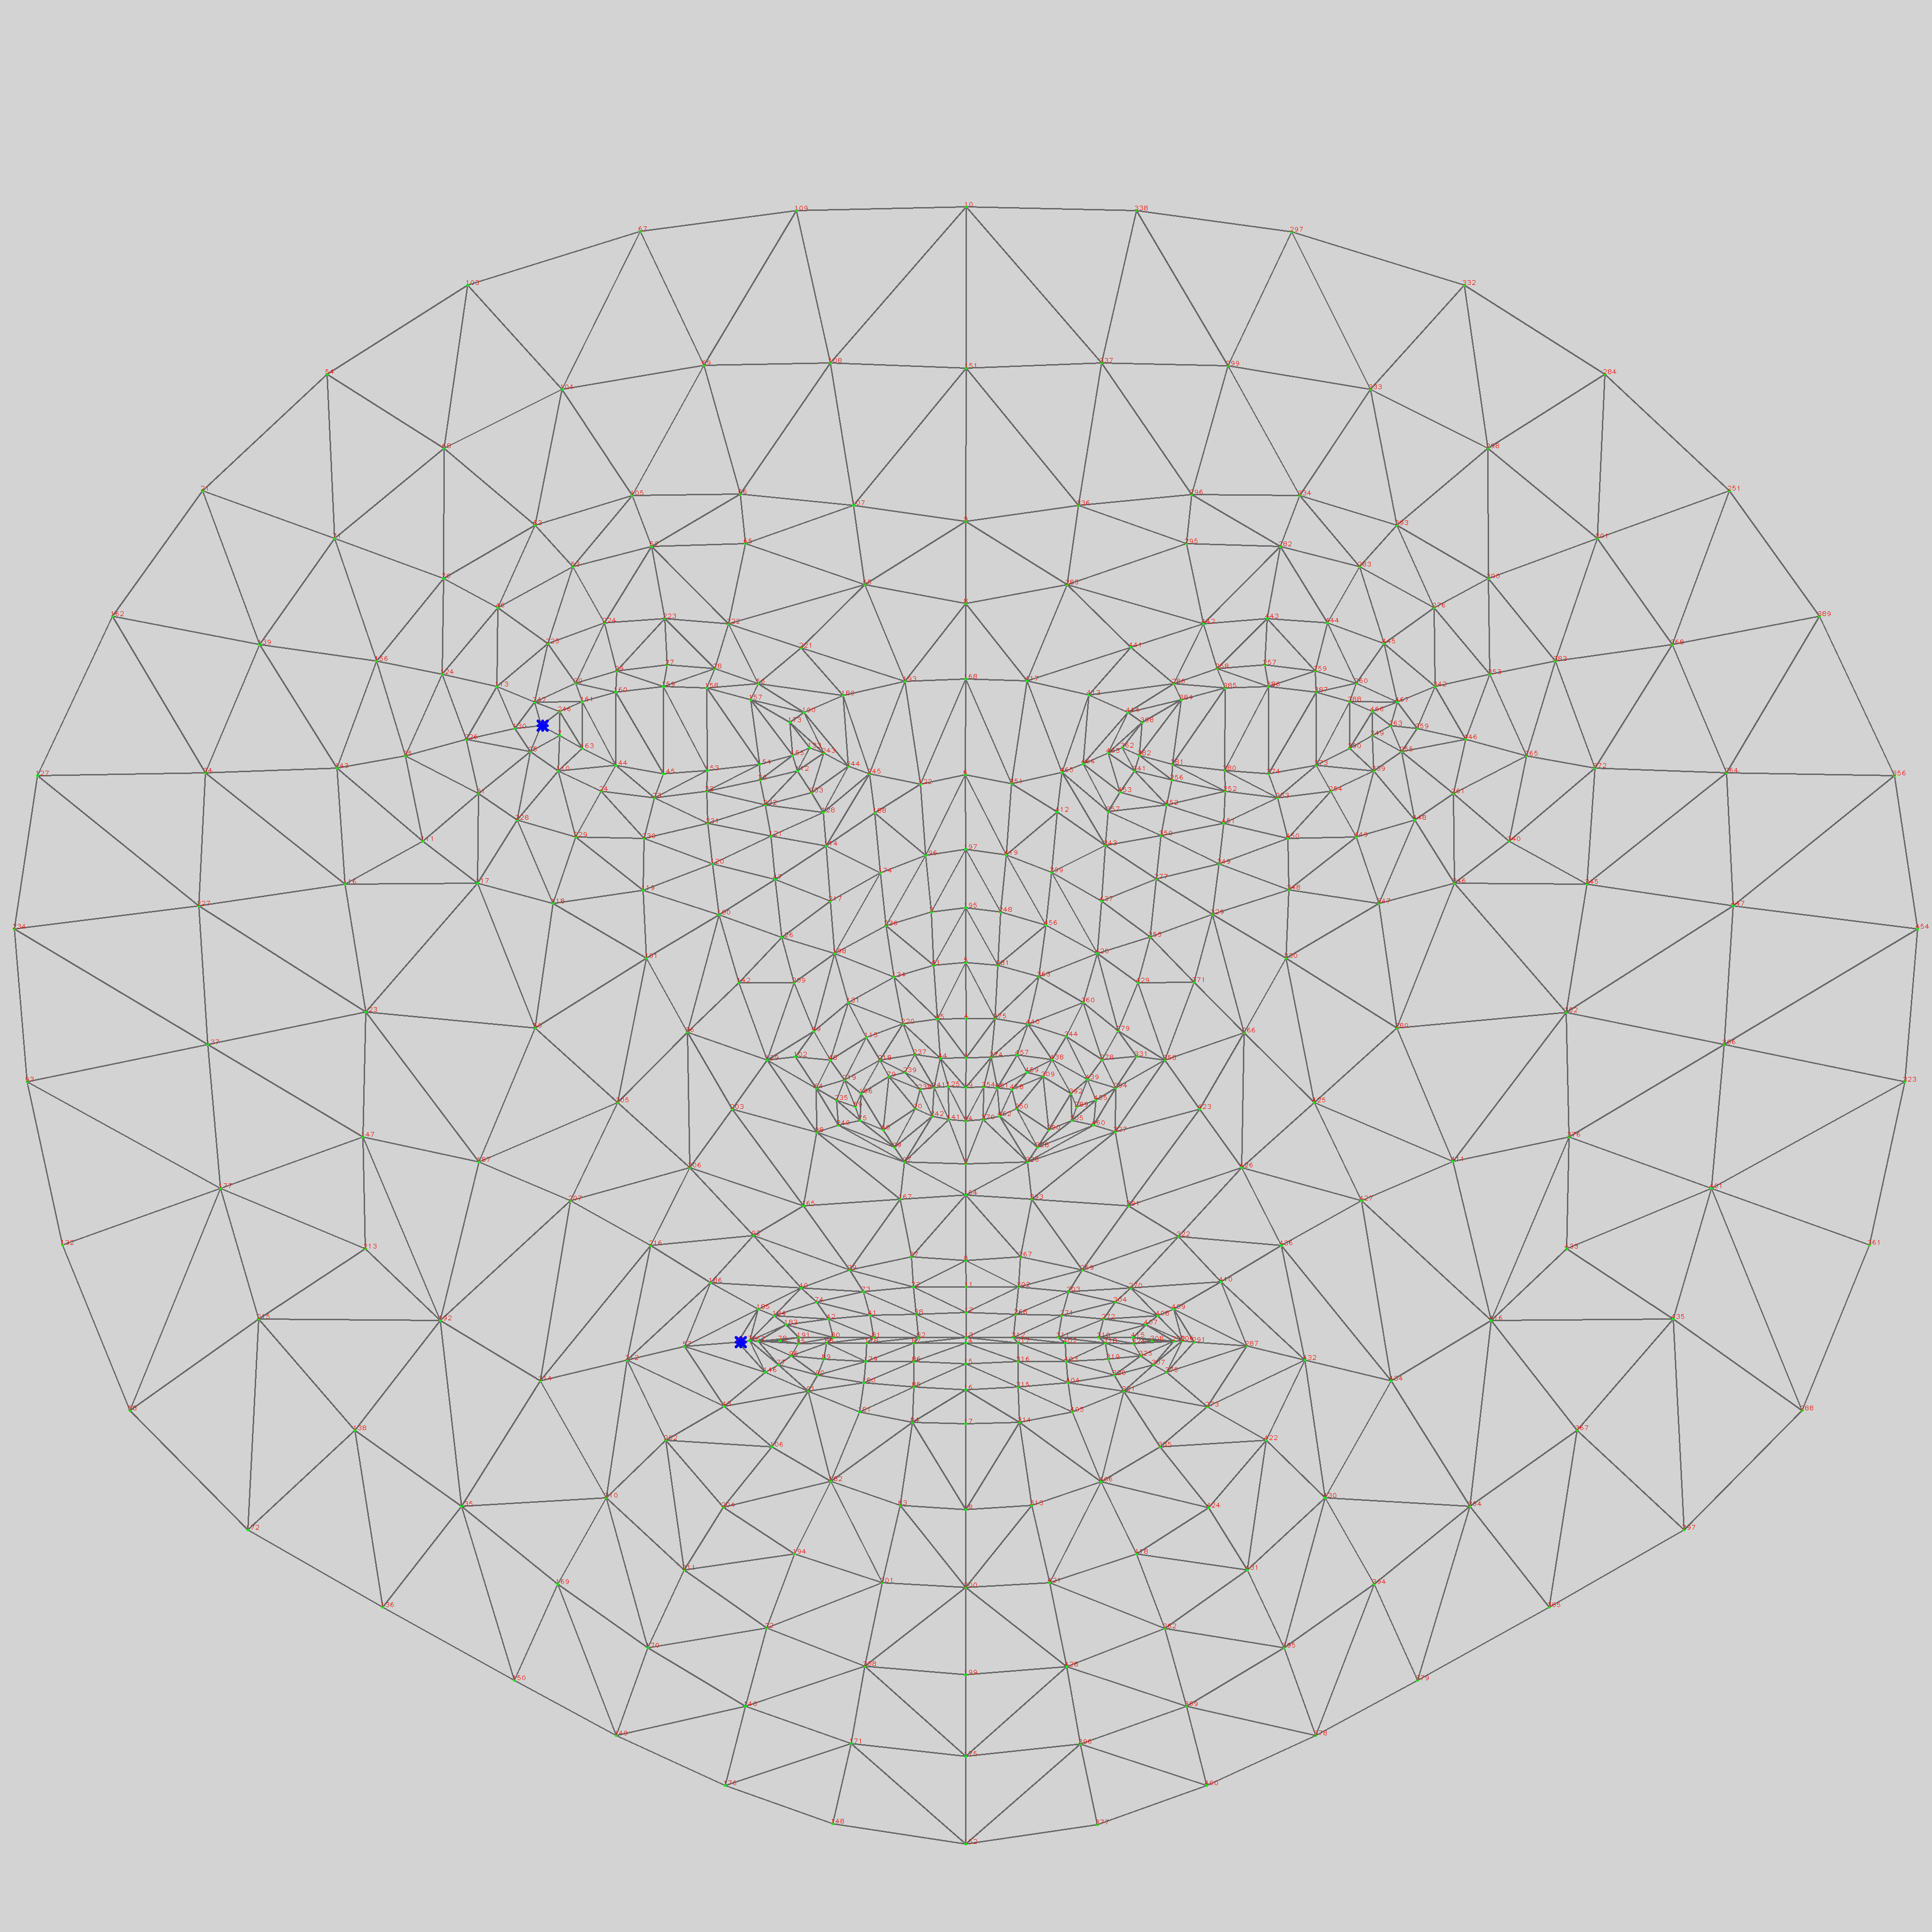
\includegraphics[scale=0.1]{figures/test.png}
    \caption{ランドマーク}
    \label{three}
  \end{center}
\end{figure}

\subsection{結果}
0°の場合の座標の差を\hyperref[four]{表\ref{four}}に、15°の場合の座標の差を\hyperref[five]{表\ref{five}}に、
30°の場合の座標の差を\hyperref[six]{表\ref{six}}に、45°の場合の座標の差を\hyperref[seven]{表\ref{seven}}に示す。
なお、今回は代表して鼻上部、顔上部、目の右端、左端の四点の座標を示す。
\begin{table}[ht!]
  \begin{center}
    \begin{tabular}{lrrrr}
       & 鼻上部(6) & 顔上部(10) & 目左端(33) & 目右端(263) \\
      x座標 & 4.869 & -0.292 & -1.739 & 1.934 \\
      y座標 & 1.175 & -2.983 & -6.414 & -7.382
    \end{tabular}
    \caption{0°の場合の誤差}
    \label{four}
  \end{center}
\end{table}
\begin{table}[ht!]
  \begin{center}
    \begin{tabular}{lrrrr}
       & 鼻上部(6) & 顔上部(10) & 目左端(33) & 目右端(263) \\
      x座標 & 5.187 & 3.612 & 2.469 & 5.693 \\
      y座標 & -1.110 & -2.077 & -1.613 & -1.804 
    \end{tabular}
    \caption{15°の場合の誤差}
    \label{five}
  \end{center}
\end{table}
\begin{table}[ht!]
  \begin{center}
    \begin{tabular}{lrrrr}
       & 鼻上部(6) & 顔上部(10) & 目左端(33) & 目右端(263) \\
      x座標 & 4.964 & 4.226 & 2.027 & 5.235 \\
      y座標 & -4.593 & 1.438 & -0.933 & -3.267 
    \end{tabular}
    \caption{30°の場合の誤差}
    \label{six}
  \end{center}
\end{table}
\begin{table}[ht!]
  \begin{center}
    \begin{tabular}{lrrrr}
       & 鼻上部(6) & 顔上部(10) & 目左端(33) & 目右端(263) \\
      x座標 & -14.728 & -4.057 & -0.012 & 1.299 \\
      y座標 & -12.880 & -12.907 & -0.954 & 4.130
    \end{tabular}
    \caption{45°の場合の誤差}
    \label{seven}
  \end{center}
\end{table}

実際には完全に同位置同姿勢で計測できているわけではないので多少の誤差はあるが、0°から30°までは誤差が小さく、
45°の場合、一部のランドマークで誤差がかなり大きくなっていることがわかる。
また実際にプログラムの動作を見た感想としても、0°から30°まではモデルがおおよそ想定通りの位置に表示されるが、それ以上の角度になると誤った大きさや角度で表示されてしまう。

\section{現時点でのマスクなし顔画像再現の様子}
現時点でのマスクなし顔画像の再現の様子を示す。
\begin{figure}[!ht]
  \begin{tabular}{cc}
    \begin{minipage}[t]{0.45\hsize}
      \centering
      \includegraphics[keepaspectratio, scale=0.4]{figures/result/mask_0.png}
      \caption{0°}
    \end{minipage} &
    \begin{minipage}[t]{0.45\hsize}
      \centering
      \includegraphics[keepaspectratio, scale=0.4]{figures/result/mask_15.png}
      \caption{15°}
    \end{minipage}
  \end{tabular}
\end{figure}
\begin{figure}[!ht]
  \begin{tabular}{cc}
    \begin{minipage}[t]{0.45\hsize}
      \centering
      \includegraphics[keepaspectratio, scale=0.4]{figures/result/mask_30.png}
      \caption{30°}
    \end{minipage} &
    \begin{minipage}[t]{0.45\hsize}
      \centering
      \includegraphics[keepaspectratio, scale=0.4]{figures/result/mask_45.png}
      \caption{45°}
    \end{minipage}
  \end{tabular}
\end{figure}
これらの画像を見てもわかるように、0°から30°まではモデルがおおよそ想定通りの位置に表示されるが、それ以上の角度になると誤った大きさや角度で表示されてしまう事がわかる。

\section{顔認識ライブラリの比較}
これまではマスクあり顔画像の特徴点を検出する顔認識ライブラリとしてMediapipeのFaceMeshを利用していたが、他の顔認識ライブラリを用いることで、
マスク越しの顔認識の性能を向上させることができるのではないかと考えた。性能を比較する顔認識ライブラリとしてOpenCVのFace Recognition、MTCNN、
MediapipeのFace Detection、InsightFaceを用いた。それぞれの顔認識を用いた場合の実行速度と、
顔の向きごとにマスク越しで顔を検出できたかについて、\hyperref[eight]{表\ref{eight}}に示す。

\begin{table}[ht!]
  \begin{center}
    \begin{tabular}{lrrrrr}
       & 実行時間 & 0° & 20° & 40° & 80° \\
      Face Recognition & 0.294 & 不可 & 不可 & 不可 & 不可 \\
      MTCNN & 0.708 & 安定しない & 不可 & 不可 & 不可 \\
      Face Detection & 0.0340 & 可 & 可 & 可 & 不可 \\
      InsightFace & 0.356 & 可 & 可 & 可 & 可
    \end{tabular}
    \caption{顔認識ライブラリの比較}
    \label{eight}
  \end{center}
\end{table}
Face RecognitionとMTCNNはどの角度でも安定してマスク越しの顔認識を行うことができなかった。また、実行時間が一番早かったのはFace Detectionで、Face meshとおおよそ同じ実行時間だった。
性能が一番良かったのはInsightFaceで、45°の場合でも安定してマスク越しに顔認識をすることができたが、特徴点の座標については正確ではないため、実際にカメラ位置姿勢計算に用いる場合は修正する必要がある。
画像のサイズを落とすことで、もう少し実行速度の向上が見込めるが、これらの結果を参考すると、顔の向きが45°以下の場合はFace Meshを用いて顔認識し、それ以上の角度の場合は
InsightFaceを併用していく手法についても検討できる。 \\
参考として、Face DetectionとInsightFaceの顔認識の実行結果について下に示す。
\begin{figure}[!ht]
  \begin{tabular}{cc}
    \begin{minipage}[t]{0.45\hsize}
      \centering
      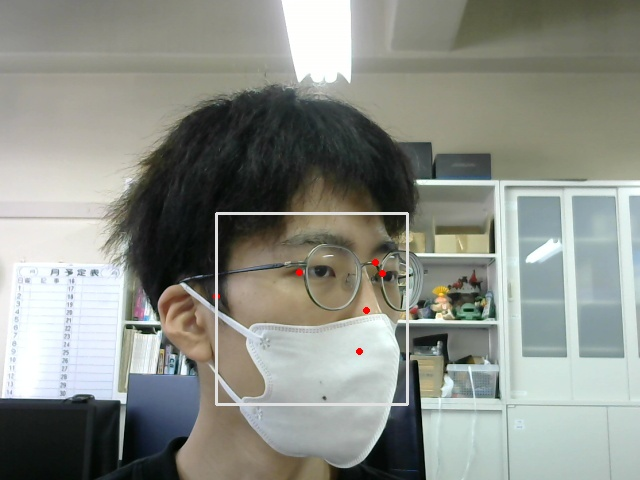
\includegraphics[keepaspectratio, scale=0.4]{figures/model/facedetection3.jpg}
      \caption{Face DEtection(40°)}
    \end{minipage} &
    \begin{minipage}[t]{0.45\hsize}
      \centering
      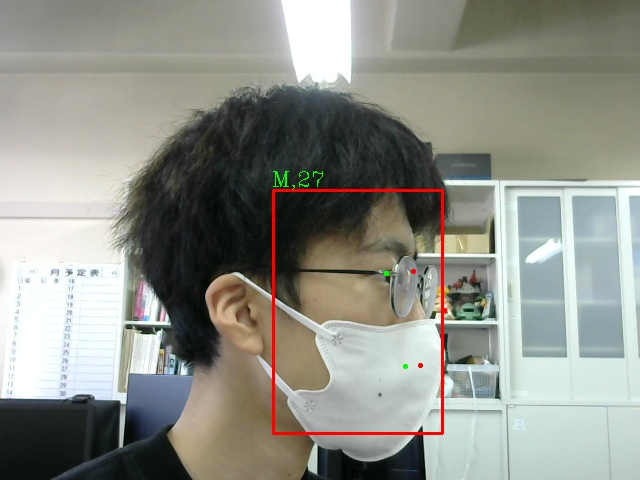
\includegraphics[keepaspectratio, scale=0.4]{figures/model/insightface4.jpg}
      \caption{InsightFace(80°)}
    \end{minipage}
    \label{nine}
  \end{tabular}
\end{figure}

\section{12月までの目標}
12月までの目標について以下にまとめる。\\
\begin{itemize}
  \item より正確な座標のずれを求める方法を考える。
  \item 顔向きの角度が一定以上の時、ランドマークの値を修正する。
\end{itemize}
%参考文献
\end{document}
